% sec_d3.tex (HT3dPert, 2026-10-14, second version; edited by HT1dPert 2026-10-15 for the note review, facts from
% HT3dPert): d = 3 perturbative HT. Numbers: numbers_d3.tex; table tab_d3_coeffs.tex (code/lri_3d_hpc/public/note_d3.py);
% figure fig_d3_c4.pdf (code/lri_3d_c4_exact/public/note_fig_d3.py); reproduction rows: repro_d3.tex; package rows:
% packages_d3.tex; checks and caveats: checks_d3.tex, caveats_d3.tex.
\section{Results in three dimensions}\label{htp:d3:sec}

\paragraph{Model and cutoff.}
In $d=3$ the generalized free field is quantized on $S^2$ (Sec.~\ref{htp:sec:method}, Ref.~\cite{htp:Hogervorst:2014rta}). A
mode $(n,\ell,m)$ has energy $\Ds+2n+\ell$, with $\ell$ the angular momentum; the zero mode $n=\ell=0$ is the local
oscillator, and all other modes form the bath. We keep the states with bath level
\begin{equation}
 N_b=\sum_{(n,\ell,m)\neq(0,0,0)}(2n+\ell)\,n_{n\ell m}\le L
 \label{htp:d3:eq:cutoff}
\end{equation}
and do not truncate the zero mode. The perturbation is $H=H_0+r\,M+g\,V$ with
$M=\int d\Omega\,{:}\phi^2{:}/(4\pi)$ and $V=\int d\Omega\,{:}\phi^4{:}/(48\pi)$. $r$ and $g$ are tuned order by order
to $E_1-E_0=\Ds$ and $E_3-E_0=3-\Ds$, and
\begin{equation}
 \DE(\eps;L)=E_2-E_0=\tfrac32-\tfrac{\eps}{6}+\sum_{n\ge2}C_n(L)\,\eps^n,\qquad \Ds=\frac{3-\eps}{4}.
 \label{htp:d3:eq:Cn}
\end{equation}
The continuum values $C_n^{(3)}$ are those of Table~\ref{htp:tab:refvals}.

\paragraph{Two codes.}
The production package (\code{code/lri\_3d\_hpc/}) builds the truncated Hamiltonian explicitly in the SO(3)-scalar,
inversion-even sector and solves the Rayleigh--Schr\"odinger recursion through $\eps^8$ in x87 long double. It reached
$L=16$, 18 and \HTpThreeLmax{} (\NThreeScalarTwenty{} scalar bath states at $L=20$, from \NThreeStatesTwenty{} before
the projection; about \NThreeSU{} service units on SDSC Expanse, charge units of about one per core-hour, with
large-memory jobs charged more). It implements two prescriptions: raw, and the vacuum window
$D_L(N_b)=E_v(L)-E_v(L-N_b)$.

The exact-sum package (\code{code/lri\_3d\_c4\_exact/}) evaluates the same coefficients as sums over intermediate states,
with exact partial-wave reductions on $S^2$ and exact zero-mode projections, at every even $L$:
\begin{itemize}
\item $C_2$ to $L=\HTpThreeLwin$, $C_3$ and $C_4$ to $L=\HTpThreeLfour$, $C_5$ to $L=\HTpThreeLfive$;
\item every window shift to $L=\HTpThreeLwin$;
\item every window scheme, including the complete window of $d=2$ (Sec.~\ref{htp:d2:sec}).
\end{itemize}
At every even $L\le20$ the two codes agree on $C_2$ to $C_5$, $r$, $g$ and the reference energies $E_0$ to $E_3$ to
$\NThreeValPkg$. The window schemes that the production package lacks agree with a brute force, built as explicit
operators on the package's own Hamiltonian at $L\le14$, to $\NThreeValBrute$. Table~\ref{htp:d3:tab:coeffs} gives the
production values.

% tab_d3_coeffs.tex: generated by code/lri_3d_hpc/public/note_d3.py from data/HT_3d/pert3d/results (do not edit)
\begin{table}[ht]\centering\footnotesize\setlength{\tabcolsep}{3pt}
\begin{tabular}{@{}l lll lll@{}}\toprule
 & \multicolumn{3}{c}{consistent (vacuum window $D_L$)} & \multicolumn{3}{c}{raw}\\
\cmidrule(lr){2-4}\cmidrule(lr){5-7}
 & $L=16$ & $L=18$ & $L=20$ & $L=16$ & $L=18$ & $L=20$\\\midrule
$C_2$ & 0.1799805130 & 0.1801641045 & 0.1803065210 & 0.1799805130 & 0.1801641045 & 0.1803065210\\
$C_3$ & $-$0.3238079917 & $-$0.3271370505 & $-$0.3298433574 & $-$0.3238079917 & $-$0.3271370505 & $-$0.3298433574\\
$C_4$ & 0.7154707349 & 0.7295143865 & 0.7400078407 & 0.7082381633 & 0.7206323697 & 0.7293066716\\
$C_5$ & $-$3.157412985 & $-$3.274129748 & $-$3.376315158 & $-$3.173233312 & $-$3.292870751 & $-$3.398184422\\
$C_6$ & 15.68169942 & 16.38726028 & 17.03798989 & 15.67552153 & 16.38079206 & 17.03198660\\
$C_7$ & $-$84.42870757 & $-$88.02482107 & $-$91.14377531 & $-$84.17501495 & $-$87.66743530 & $-$90.65688526\\
$C_8$ & 548.2872011 & 578.4398685 & 605.8501134 & 548.2146549 & 578.3577582 & 605.7652262\\
\bottomrule\end{tabular}
\caption{Finite-cutoff coefficients $C_n(L)$ in $d=3$ from the production package \code{lri\_3d\_hpc} (10 significant digits; the records hold 20), raw and with the vacuum window $D_L$. $C_2$ and $C_3$ do not depend on the window. The exact sums reproduce $C_2$ to $C_5$ of this table to $3\times10^{-13}$; from $C_4$ on, neither scheme converges (Fig.~\ref{htp:d3:fig:c4}).}
\label{htp:d3:tab:coeffs}\end{table}


\paragraph{The vacuum window diverges at $\eps^4$.}
$C_2(L)$ and $C_3(L)$ do not depend on the window and converge. From $C_4$ on, the vacuum window does not suffice
(Fig.~\ref{htp:d3:fig:c4}).
\begin{itemize}
\item As in $d=2$, divergent sub-bubbles inside a state see only the level left by the other quanta, while $r$, $g$ and
 the vacuum are tuned with the full $L$.
\item In $d=3$ the mass sub-bubble diverges like $L^{3/2}$ instead of $L$, so every term is one power worse.
\item Uncorrected, $C_4(L)$ falls like $-\NThreeRawLsq\,L^2$.
\item With $D_L$ alone it peaks at $\NThreeCfourConsPeak$ near $L=32$ and is $\NThreeCfourConsSix$ at $L=600$. The
 terms are $-\NThreeConsLin\,L$ and $-\tfrac{10}{243\,\Gamma(7/2)}\sqrt L\ln L$, which the diagonal and
 zero-mode-number-changing parts of the zero-mode window remove.
\item The mass window ($\chi$-attached sunset term), which in $d=2$ is a finite shift, here removes a further
 $\NThreeChiSqrt\sqrt L$.
\end{itemize}

\paragraph{Complete window.}
The complete window $W$ of $d=2$ is carried over unchanged: vacuum window, full zero-mode window, and mass window
$-\tfrac12 r_2'(L)\{\hat N_b,M'\}$, with $\hat N_b$ the bath-level operator. With it, $C_4(L)$ converges like $1/L$. At
$L=600$ it is $\NThreeCfourWsix$. With the limit fixed at $C_4^{(3)}$, a free $\sqrt L$ term comes out below
$\NThreeNoDiv$. The mass window is used in its leading-order linear form; since $r_2$ is not linear in $L$ in $d=3$, the
exact form may differ by a finite amount, which the agreement below suggests is small but which is not derived.

At $\eps^5$ the nested windows are referred to the outer cutoff (rule $W_c$ of $d=2$); the external-line window
($W_{cs}$) changes $C_5(40)$ by $-0.003$.

\begin{figure}[ht]\centering
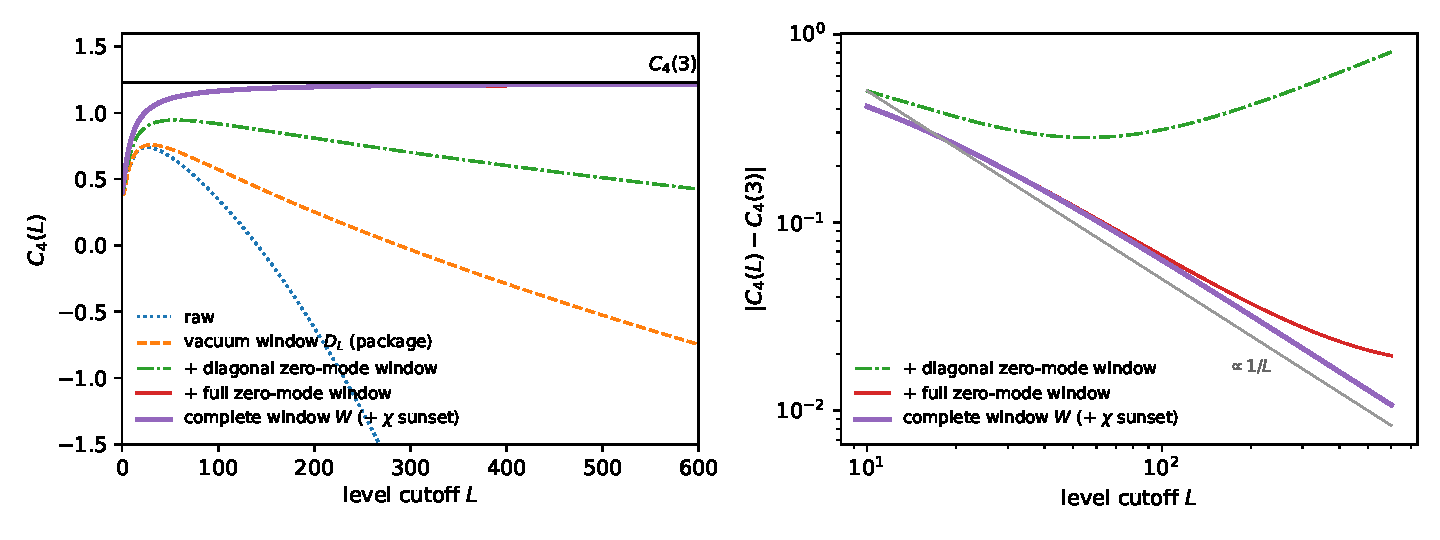
\includegraphics[width=\linewidth]{parts/htp/sections/d3/fig_d3_c4.pdf}
\caption{$C_4(L)$ in $d=3$ from the exact sums, in each window scheme. Left: raw, the vacuum window $D_L$ of the
production package, and the zero-mode and mass windows added one by one (the full-zero-mode curve lies under $W$ at this
scale). Right: distance from $C_4^{(3)}$ on logarithmic axes. The complete window $W$ converges like $1/L$; without its
mass window the distance stops decreasing, has its minimum near $L\approx1100$ and grows like $3.6\times10^{-4}\sqrt L$
beyond the plotted range.}
\label{htp:d3:fig:c4}
\end{figure}

\paragraph{Extrapolations.}
Fit forms (towers of $L^{-k}\ln^jL$ terms, from the $d=2$ protocol) and windows were chosen after the data were seen,
with the continuum values known; the quoted uncertainties are spreads over fits, not standard errors.
\begin{itemize}
\item $C_2=\HTpCtwoThree$ ($\HTpCtwoThreeDigits$ digits of the closed form; fit to $L\le\HTpThreeLwin$).
\item $C_3=\HTpCthreeThree$ ($\delta=\HTpCthreeThreeDev$): mean and half-range of three fit windows.
\item $C_4=\HTpCfourThree$ ($\delta=\HTpCfourThreeDev$): median of one tower over 12 fit windows; the uncertainty is
 the half-range, including a blind fit to $L\le400$ that predicts $402\le L\le600$ to $\NThreeCfourBlind$. Towers with
 one more correction term spread to about $10^{-4}$.
\item $C_5$, provisional and calibrated on $C_4^{(3)}$: towers are kept if, on $C_4^W(L)$ at the same $L\le40$, they
 reproduce $C_4^{(3)}$ to within 0.036 and pass a blind test. The median of their $C_5$ fits gives $\HTpCfiveThree$
 (median $\NThreeCfiveMed$) against $C_5^{(3)}=-5.850351421$. The uncertainty is the worst $C_4$ miss relative to the
 remaining $C_4$ correction at $L=40$ (0.036 of 0.147), times the remaining $C_5$ correction at $L=40$ (1.28, which
 uses $C_5^{(3)}$ itself).
 \begin{itemize}
 \item This is a weak test: $C_5^{W_c}(40)=\NThreeCfiveWcForty$ is still 1.28 above the limit.
 \item A term in $L^{-1/2}$, which $L\le40$ cannot exclude, would lower the limit by 0.5 to 1.
 \item A window without the mass window also fits at $L\le40$, although it differs from $W_c$ by a term growing like
  $L^2$.
 \item Going further needs a new representation of the angular channels: the cost grows like $L^{8.4}$ and the memory
  like $L^{4.5}$.
 \end{itemize}
\end{itemize}

\paragraph{Descendant spacings.}
For the scalar descendant of $\phi$ (the $n=1$, $\ell=0$ quantum), the window removes the $\eps^2$ violation of its
spacing as $L\to\infty$. At $\eps^3$ the external-line window acts in the right direction, but the violation is not shown
to vanish at $L\le16$.
